\documentclass{article}

%maths
\usepackage{mathtools}
\usepackage{amsmath}
\usepackage{amssymb}
\usepackage{amsfonts}

%tikzpicture
\usepackage{tikz}
\usepackage{scalerel}
\usepackage{pict2e}
\usepackage{tkz-euclide}
\usetikzlibrary{calc}
\usetikzlibrary{patterns,arrows.meta}
\usetikzlibrary{shadows}
\usetikzlibrary{external}

%pgfplots
\usepackage{pgfplots}
\pgfplotsset{compat=newest}
\usepgfplotslibrary{statistics}
\usepgfplotslibrary{fillbetween}

%colours
\usepackage{xcolor}

\begin{document}

Example of a line drawn using TikZ:
\\

\begin{center}
    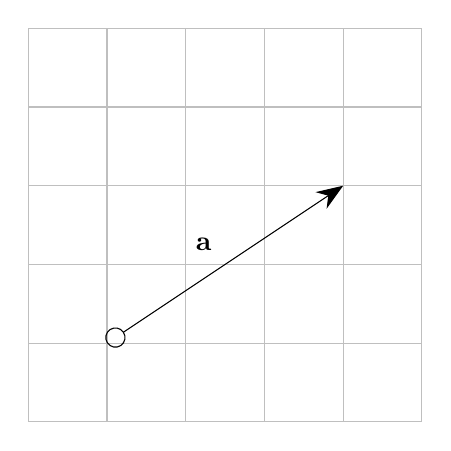
\begin{tikzpicture}
        \draw[lightgray] (0,0) grid (5,5);
        \draw[{Circle[scale=2,open]}-{Stealth[scale=2]}] (1,1) -- (4,3)
        node[midway,above left=2pt,rotate=0] {$\mathbf{a}$};
    \end{tikzpicture}

\end{center}

A circle of radius $0.1$ centered at $(1,1)$ and a rectange:
\\

\begin{center}
    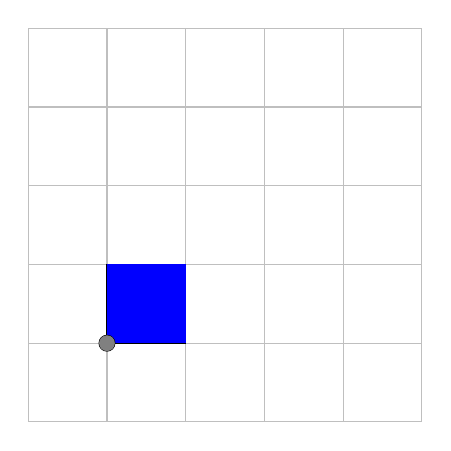
\begin{tikzpicture}
        \draw[lightgray] (0,0) grid (5,5);

        \draw (1,1) rectangle (2,2);
        \fill[blue] (1,1) rectangle (2,2);

        \draw (1,1) circle [radius=0.1];
        \fill[gray] (1,1) circle [radius=0.1];
    \end{tikzpicture}

\end{center}

An arc:
\\

\begin{center}
    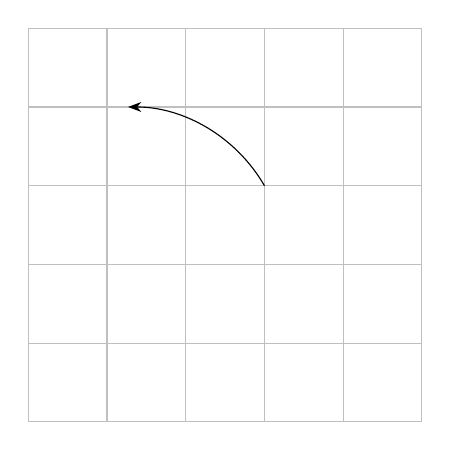
\begin{tikzpicture}
        \draw[lightgray] (0,0) grid (5,5);

        \coordinate (A) at (3,3);

        \draw[-Stealth] (A) arc (30:90:2);    %(30:90:2) = (start-angle:end-angle:radius)
    \end{tikzpicture}
\end{center}

Venn diagrams:
\\

\begin{center}
    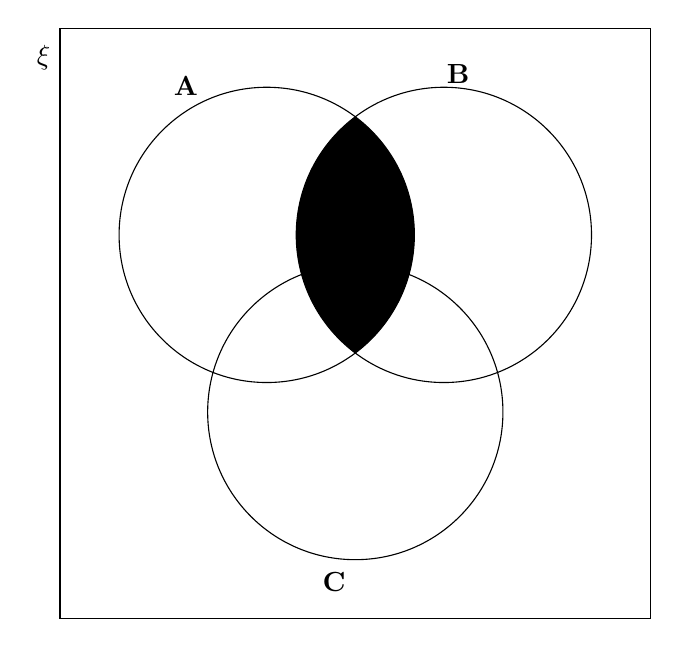
\begin{tikzpicture}[scale=1.5]
        \coordinate (C1) at (0,0);
        \coordinate (C2) at (1.5,0);
        \coordinate (C3) at (0.75,-1.5);
        \coordinate (R1) at (-1.75,-3.25);
        \coordinate (R2) at (3.25,1.75);

        \draw (C1) circle (1.25);
        \draw (C2) circle (1.25);
        \draw (C3) circle (1.25);

        \draw (R1) rectangle (R2);

        \coordinate [label=left:$\xi$] (R) at (-1.75,1.5);
        \coordinate [label=above left:\textbf{A}] (A) at (-0.5,1.1);
        \coordinate [label=above left:\textbf{B}] (B) at (1.8,1.2);
        \coordinate [label=above left:\textbf{C}] (C) at (0.75,-3.1);

        \clip (C1) circle (1.25);
        \fill (C2) circle (1.25);
    \end{tikzpicture}
\end{center}

Plotting graphs:
\\

\pgfplotsset{
    standard/.style={
    axis line style = thick,
    trig format=rad,
    enlargelimits,
    axis x line=middle,
    axis y line=middle,
    enlarge x limits=0.15,
    enlarge y limits=0.15,
    every axis x label/.style={at={(current axis.right of origin)},anchor=north west},
    every axis y label/.style={at={(current axis.above origin)},anchor=south east},
    }
}

\begin{center}
    \begin{tikzpicture}
        \begin{axis}[standard,
            xtick={-0.3,0.2},
            ytick=\empty,
            xlabel={$x$},
            ylabel={$y$},
            samples=1000,
            xmin=-0.52, xmax=0.4,
            ymin=-0.05, ymax=0.55
            ]
            
            \node[anchor=center,label=south west:$O$] at (axis cs:0,0){};

            \addplot[name path=F,domain={-0.5:0.38158}]{(sin(e^(3*x))*e^(3*x))/(cos(e^(3*x))+4)};
            \addplot[name path=G,domain={-0.5:0.38158}]{-x^2};
            \path[name path=xAxis] (axis cs:-0.3,0) -- (axis cs:0.2,0);
            \addplot[fill=blue,fill opacity=0.2,] fill between [of=F and G,
            soft clip={domain=-0.3:0.2}];
        \end{axis}
    \end{tikzpicture}
\end{center}
\end{document}